\section{Experiment Set-up}\label{Sec:Exp}

In this section we give an overview on the data used for the experiment, its processing and how it was split. More importantly, we outline the specifications of the modeling process and the evaluation method for performance assessment. 

\subsection{Data Sets and Preprocessing}

To conduct our experiment we use four credit scoring data sets. There are on the one hand two data sets obtained from \textit{Kaggle}: the 2010 \textit{PAKDD data mining challenge} data set\footnote{ \url{https://www.kaggle.com/c/pakdd2010-dataset/}}  (PAK) and the \textit{Give Me Some Credit competition} data set\footnote{ \url{http://www.kaggle.com/c/GiveMeSomeCredit}} (GMC). On the other hand we make use of two well-known UCI Machine Learning Library data sets, the \textit{Default of Credit Card Clients} data set (TCD) from Taiwanese bank customers \citep{yeh2009comparisons} and the \textit{South German credit} data set (GER), which is a reviewed version of the very common \textit{German credit} data set \citep{groemping2019south}. A brief overview on the data is given in Tab. \ref{tab:ov}. Each data set contains customer data from financial institutions. All sets are composed of a mixture of socio-economic information from the customer (i.e. age, education, maritial status), information from their loan inquiry (i.e. amount, duration) and an assessment of whether the customer failed to repay his loan. 

\begin{table}[!htb]
	\begin{center}
		\small
		\begin{tabularx}{0.95\textwidth}{@{} l *{5}{d{2.0}} @{}}
			\toprule
			Data Set & \mc{Prior default}  & \mc{Observations} & \mc{Number of} & \mc{Number of} &  \mc{Missing} \\
			&           \MC{risk}     &                       & \MC{variables}   & \MC{selected vars.} & \MC{Values} \\
			\midrule
			GER & 0.30 & 1,000 & 21 & 16 & No \\
			GMC & 0.07 & 150,000 & 12 & 11 & Yes  \\
			PAK & 0.26 & 50,000 & 54 & 11 & Yes  \\
			TCD & 0.22 & 30,000 & 25 & 17 & No  \\
			\addlinespace
			\bottomrule
		\end{tabularx}
	\end{center}
	\caption{Overview data sets}
	\label{tab:ov}
\end{table}

The first step for data processing is to make a decision about variable selection, as our lattice models requires a low amount ($n \leq 20$) of covariates.\footnote{ In addition, the computational resources for performing the experiment were rather restriced.} The main criteria for this selection are ($i$.) correlation, see the exemplary correlation plot in Appendix Fig. \ref{Fig:corrplot}, ($ii$.) and comparability, which aims to have similar variables for all data sets. Tab. \ref{tab:ov} shows the reduction of variables for each data set. As a next step we apply standard preprocessing operations as imputation of missing values by mean/mode replacement. In addition we transform the data type of every variable to be numeric, since the lattice model requires tensor shaped input data. We do not normalize the data, as none of the models requires such an operation. For the partitioning of the data we apply a simple $80/20$ train/test split, no validation or cross validation, to keep computing effort low.

\begin{figure}[htb!]
		\centering
		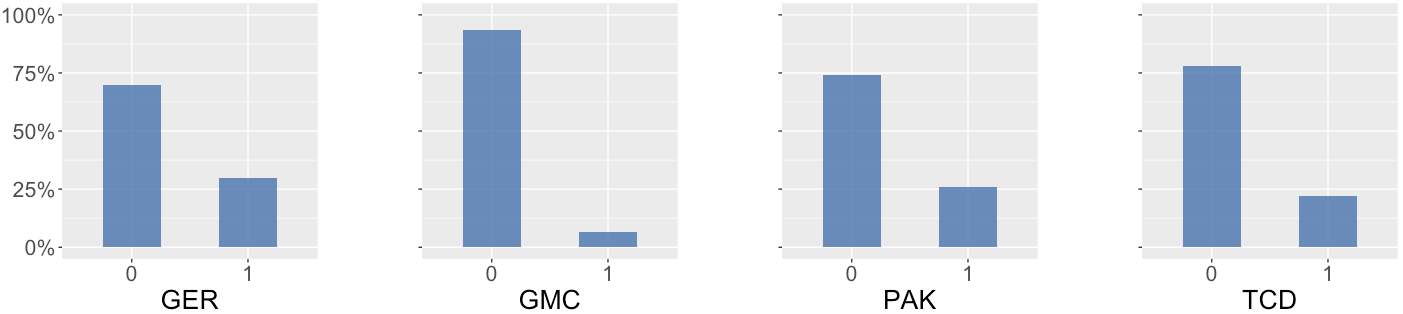
\includegraphics[width=1\textwidth]{img/defhist} % first figure itself
		\caption{The distribution of credit default for each data set.}
		\label{Fig:defhist}
\end{figure}

\subsection{Modeling and Evaluation}

The goal of this thesis is to explore lattice based models. To asses its performance, we set up an experiment in which we compare a nonlinear generalized additive model
(GAM), also referred to as lattice model, and a random forrest classifier. The algorithms are applied in a credit scoring domain on a classification problem: each of the above introduced data sets contains a binary class label for each client that determines if there is a prior risk of some kind of default or not (see Fig. \ref{Fig:defhist}). We renamed the target variable for each data set to `default' and since we are facing a binary outcome we set the value for `customer likely defaults' to $y = 1$ and for `customer likely not defaults' to $y = 0$. We chose a random forrest classifier for the comparison, as it is commonly used for credit scoring \citep{baesens2003benchmarking}, \citep{lessmann2015benchmarking}. Due to computational restrictions we forwent tuning the hyperparameters of the models. To deploy the lattice model we set up an interface to call the Tensor Flow Lattice Python library, as the experiment was run in an \textsf{R} environment. A full description of each model can be found in the accompanying \textsf{R}-script. The following gives a brief overview on the most important parameters and aspects of each model:

\subsubsection*{Calibrated Lattice Model}

Among a set of hyperparameters our, `nonlinear generalized additive model (GAM), also called a calibrated linear model in the TensorFlow Lattice' \citep[Sec.~8]{wang2020deontological}, requires a detailed specification for calibration. As we saw in Sec. \ref{Sec:cal}, a lattice model first applies piecewise-linear and categorical calibration on each input variable. The calibration function $c_d(x[d]; \alpha^{(d)})$ is parametrized by $K$ ($\alpha^{(d)} \in [0, M_d - 1]^K$, with $K$ differing for continous and categorical variables), which in simple terms determines the spacing of $c_d(\cdot)$ (\cite{gupta2016monotonic} give a detailed explanation of the calibrator on pp. 26). The amount of keypoints $K$ set and the type of spacing (by quantiles, linearly or manually) has to be specified for every variable of each data set. Our decision making about the parametrization of $c(\cdot)$ was guided by the distribution of the individual variables; if e.g. a variable had a strong skew and outliers, we would pick a higher value for $K$ and a quantile spacing. The specification for every variable and data set can be looked at in the feature configs \textsf{Python} file. 

\begin{figure}[htb!]
	\centering
	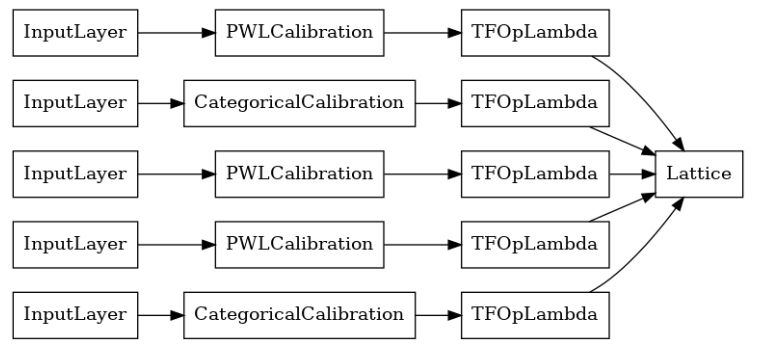
\includegraphics[width=0.65\textwidth]{img/lat}
	\caption{A simplified version of our model}
	\label{Fig:lat}
\end{figure}

There are two further important per-variable configurations entailed in this file: lattice size and monotonicity. The first we kept mostly at a default value of $2$ for the vast majority of variables, mainly to keep computational effort low. For monotonicity we again looked at variable distribution behaviour, to decide if it makes sense to apply monotonicity and whether it should be in- or decreasing. Simple charts of the variables as in Appendix Fig. \ref{Fig:ovplot} were helpful for decisions.

After calibration a lattice layer non-linearly fuses the calibrated variables, see Fig. \ref{Fig:lat}. As a regulizer for the calibration we chose the Hessian, and for making the lattice more linear we used the Torsion regulizer, both set to a value of $0.01$. Further parameters included\textit{ binary crossentropy} loss function and \textit{Adam} optimizer; a \textit{learning rate} of $0.01$, a rather large \textit{batch size} of $128$ and a rather small \textit{epoch size} of $25$, both for computational reasons.

\subsubsection*{Random Forrest}

Our random forest model of choice contains three potential tuning parameters:  a value for the number of trees, a value for the number of data points that are required for a node to split and a value for the number of predictors that will be randomly sampled at each split. We set the tree parameter at $1000$, the minimum node size parameter to $3$ and the last one at $null$. A more detailed explanation of the model can be found in \citep{breiman2001random}.

\subsubsection*{Evaluation}

Both of the introduced models were then applied to all of the credit scoring data sets. For the assessment of each classifier we chose \textit{AUC} as evaluation metric, since it is a well established metric for this kind of classification problem \citep{lessmann2015benchmarking}.

For the comparison of the performance of two classifiers on multiple datasets it is recommended to perform a statistical test on the obtained evaluation metrics, rather then just averaging over them \citep{japkowicz2011evaluating}. For our comparison of the AUC values of both models we therefore conducted \textit{Wilcoxon's Signed-Rank test}, following the approach of \citep[Sec.~6.6]{japkowicz2011evaluating}. For this test the $H_0$-hypothesis is that both classifiers perform equally as good; we are thus going to try to show, that one classifier performs better than the other one. 
\medskip

Wilcoxon's Signed-Rank test works the following way: for each pair of AUC values the difference $d_i$ is taken. These get ranked, respectively their absolute values; if a tie occurs, an average rank will be assigned to the tied values. Then a sum of ranks is calculated:
\begin{align*}
W_{s1} = \sum_{i=1}^{n} I(d_i > 0) \mathrm{rank}(d_i) + \frac{1}{2} \sum_{i=1}^{n} I(d_i = 0)\mathrm{rank}(d_i),  \\	
W_{s2} = \sum_{i=1}^{n} I(d_i < 0) \mathrm{rank}(d_i) + \frac{1}{2} \sum_{i=1}^{n} I(d_i = 0)\mathrm{rank}(d_i). 
\end{align*}

With these sums a test statistic can be calculated as $T_{wilcox}  = \mathrm{min}(W_{s1}, W_{s2}).$ To verify the rejection of $H_0$, critical values for $n < 25$ can be looked up from a table, otherwise the $T_{wilcox}$ distribution can be approximated. For a more detailed description of the test procedure see \citep[p.~234]{japkowicz2011evaluating}.
